\documentclass[12pt, fleqn]{article}

\usepackage{amsfonts,amsthm,amsopn,amssymb,latexsym}
\usepackage{graphicx}
\usepackage[pdftex]{hyperref}
\usepackage[T1]{fontenc}
\usepackage[brazil]{babel}
\usepackage[utf8]{inputenc}
\usepackage{a4wide}
\usepackage[intlimits]{amsmath}
\usepackage{multirow}
\usepackage{placeins}               
\usepackage{url}

\setlength{\textwidth}{16.0cm}        % largura do texto
\setlength{\textheight}{9.0in}        % tamanho do texto (sem head, etc)
\renewcommand{\baselinestretch}{1.15} % espa�amento entre linhas
\addtolength{\topmargin}{-1cm}        % espa�o entre o head e a margem
\setlength{\oddsidemargin}{-0.1cm}    % espa�o entre o texto e a margem

% Ser indulgente no preenchimento das linhas
\sloppy 

\begin{document}

    \pagestyle {empty}

    \vspace*{-2cm}
{\bf
\begin{center}
  {\large
  \hspace*{0cm}Universidade Federal de Juiz de Fora} \\
  \hspace*{0cm}Departamento de Ciência da Computação \\
  \hspace*{0cm}DCC059 - Teoria dos Grafos Semestre 2015-2  \\
\end{center}}
\vspace{4.0cm}
% \noindent
\begin{center}
  {\Large \bf Problema de cobertura de vértices ponderados com minimização de vértices } \\[4cm]
  {\Large Daniel André Carlos Cândido}\\[6mm]
  {\Large Professor: Stênio Sã Rosário F. Soares}\\[3.0cm]
\end{center}

{\raggedleft
\begin{minipage}[t]{8.3cm}
  \setlength{\baselineskip}{0.25in}
  Relatório da terceira parte do  trabalho de Teroria dos Grafos, parte integrante da avaliação da disciplina.
\end{minipage}\\[1cm]}

\vspace{4cm}
{\center Juiz de Fora \\[1mm]
Março de 2016 \\}

\newpage
    
    
    \pagestyle {empty}
    
    \newpage

    \pagestyle {plain}

    \setcounter{page}{0} \pagenumbering{arabic}
    
    \setlength{\parindent}{0in}  
    
    \parskip 5pt  

    \section{Introdução}

    %comando cria itens
      \par O trabalho foi desenvolvido ao longo da disciplina de Teoria dos Grafos, que consiste em apresentar um conjunto de funcionalidades que permite manipular um grafo qualquer. 
	    Foi utilizado para representado do grafo uma listas de adjacências. Esse trabalho foi dividido em duas partes, que serão explicadas no topico ``Estruturas de dados utilizadas`` 
	    (é importante salienter que as funcionalidades implenetadas na primeira parte do trabalho são incorporada na segunda parte).
	    E, os grafos analisados serão das instâncias fornecidas junto com a especificação do trabalho e uma instâncias desenvolvido pelo autor do trabalho. 


    \section{Metodologia utilizada}
      \par Dentre as linguaguens de programação propostas, C++ foi a linguagem escolhida para implementar as funcionalidades do algoritmo solicitado. 
	Pois, trata-se de uma abordagem flexível e multiparadigma permitindo ainda o uso de orientação a objetos, programação genérica e em alguns casos o uso de ambos em um mesmo código. 
	Uma outra vantagem está nos problemas relacionados à memória, visto que nesses casos é possível adotar um estilo de mais baixo nível.


      \subsection{Estruturas de dados utilizadas}	
	\par O algoritmo implementado possui as seguintes classes:
	  \begin{itemize}
	      \item Classe Grafo: Responsável pelas manipulações do grafo em si. 
	      O grafo é representado por listas de adjacências, e para cada vértice há uma lista encadeada contendo suas arestas com os demais vértices do grafo. 
	      As listas são compostas de item e são representações de grafos, logo grafos são listas, e essa relação pode portanto, ser definida como herança simples. 
	      Os vértices estão definidos como listas de arestas e itens do grafo, ou seja herança múltipla. As arestas, por sua vez, são apenas itens dos vértices o que nos faz apresentar outro exemplo de herança simples. 
	      A classe contém funções para: retornar o grau (dado um vértice como parâmetro), remover nós e arestas, adicionar nós e arestas, verificar a ordem do grafo,
	      verificar se o grafo é k-regular, verificar a quantidade de arestas o grafo possui, verificar se um grafo é completo entre outras funcionalidades descritas na próxima subseção.
	      
	      \item Classe Vértice: Utilizada para manipulações referentes às arestas. Suas funções se referem basicamente a: verificar existência de arestas,
	      encontrar arestas, e remover arestas (ambas apresentando o valor do id do vértice como parâmetro).
	      
	      \item Classe Item: Possui operações referentes à lista encadeada. Como por exemplo, pegar próximo, pegar anterior, pegar informação, entre outras.
	      
	      \item Classe Lista: Apresenta as operações referentes à lista de vértices. Como por exemplo, contar número total de itens, adicionar e deletar item, entre outras.
	      
	      \item Classe LeituraGravacao: Responsável pela leitura e gravação dos arquivos de texto. Sendo que os arquivos de leitura são as instâncias contendo os grafos. 
	  \end{itemize}

      \subsection{Funções implementadas na primeira parte}
	\par Na primeira parte do desenvolvimento do trabalho, 
	    foi implementadas funcionalidades basicas para a manipulações do grafo e outras funcionalidades que serão citadas abaixo. 

      \begin{itemize}
	\item Fucionalidades Basicas:
	  \begin{itemize}
	      \item Leitura e escrita de aquivos.
	      \item Adição e remoção de nos.
	      \item Adição e remoção de arestas.
	      \item Retornar o grau do nó.
	      \item Verificar a k-regularidade do grafo, aonde o k é informado pelo usuário.
	      \item Informar a ordem do grafo.
	      \item Verificar se o grafo é trivial.
	      \item Verificar se o grafo é nulo.
	      \item Retornar o grau do grafo.
	  \end{itemize}
	  
	\item Funcionalidades Intermediárias:
	  \begin{itemize}
	      \item Mostra a vizinhaça aberta de um nó.
	      \item Mostra a vizinhaça fechada de um nó.
	      \item Verificar se o grafo é um multtgrafo.
	      \item Verificar se o grafo é completo.
	      \item Verificar se o grafo é bipartido.
	      \item Encontrar o menor caminho entre dois vértice(Utilizando o Dijkstra).
	  \end{itemize}
      \end{itemize}

      \newpage

      \subsection{Funções implementadas na segunda parte}
      \par Na segunda parte do desenvolvimento do trabalho pratico, foram implementadas funções para manipular árvore geradora mínima e busca.
      %Foram elaborados algoritmos de Kruskal e Prim, Fecho Transitivo Direto, Fecho Transitivo Indireto, Clique Máxima e Componente Fortemente Conexa.
	\begin{itemize}
	    \item Algoritmo de Kruskal e Algoritmo de Prim: Consistem em encontrar uma árvore geradora mínima em um grafo conexo.
	    \item Busca em largura e pefundidade: Consiste em encontrar um dado vértice v no grafo. 
	    \item Algoritmo de Flody-Warshall: Consiste em encontrar o menor valor do caminho de um vértice v para todos os vétices u do grafo.
	\end{itemize}

      \subsection{Abordagens utilizadas}
	\par A abordagem utilizada para o desenvolvimento do trabalho é a lista de adjacência e lista encadeada para manter as relações entre vértices e arestas. 
	Em algumas funções, foi utilizada fila de prioridade, algoritmo de ordenação  ''sort`` que utiliza o Quicksort para ordenação e a classe vector, onde todas as estruturas são da propria linguagem. 

    \section{Experimentos computacionais}
      \par As funções implementadas foram desenvolvidas e testadas em computadores com sistema operacional Linux com as seguintes especificações.
      \begin{itemize}
	  \item Processador: AMD FX 6300.
	  \item Placa de Video: GeFoce GTX960.
	  \item Menoria RAM: 12GB DDR3.
      \end{itemize}
      \par Como mencionado anteriormnete, as instâncias utilizadas formato .txt foram fornecidas junto com a especificação do trabalho e desenvolvida pelo autor do trabalho. 
	Os resultados que serão mostrado a seguir, foi utilizado a instância ''teste.txt`` desenvolvida pelo autor do trabalho como mostrado na imagem abaixo.	
      
      \begin{figure}[!htpb]
	  \centering
	  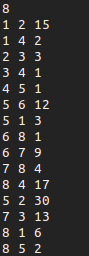
\includegraphics[scale=0.8]{instacia.png}
	  \caption{Instância: teste.txt}
	  \label{fig:Instância: teste.txt}
      \end{figure}     
      
       
    \newpage
      
      \par Resultados:
      \begin{itemize}
	\item Algoritmo Flody-Warshall:
	  \begin{figure}[!htpb]
	    \centering
	    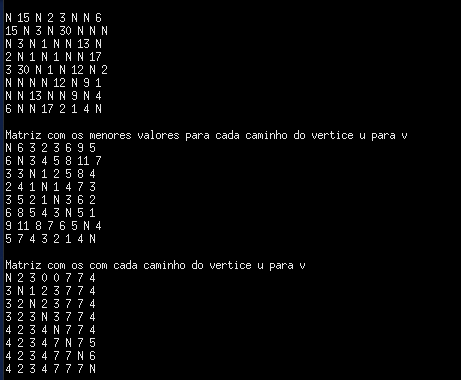
\includegraphics[scale=0.8]{floyd.png}
	    \caption{Algoritmo Flody-Warshall, a primeira matriz sem a execução do algoritmo, a segunda e resuldado do algoritmo 
		    e a terceira represeta o menor caminho do vértice v para cada vértice u}
	    \label{fig:Flody}
	  \end{figure}
	\newpage
	\item Algoritmo Prim:
	  \begin{figure}[!htpb]
	    \centering
	    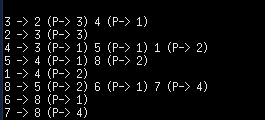
\includegraphics[scale=0.9]{prim.png}
	    \caption{Arvore geradora mínima resultante do algoritmo Prim}
	    \label{fig:prim}
	  \end{figure}
	
	\item Algoritmo Kruskal:
	  \begin{figure}[!htpb]
	    \centering
	    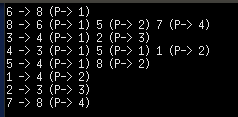
\includegraphics[scale=0.9]{kruskal.png}
	    \caption{Arvore geradora mínima resultante do algoritmo Kruskal}
	    \label{fig:kruskal}
	  \end{figure}
	  
	\item Algoritmo Dijkstra:
	  \begin{figure}[!htpb]
	    \centering
	    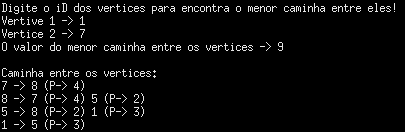
\includegraphics[scale=0.9]{dijkstra.png}
	    \caption{Menor valor e o caminho entre dois vértice utilizando o algoritmo Dijkstra}
	    \label{fig:dijkstra}
	  \end{figure}
	  
      \end{itemize}

    \newpage
    \section{Conclusões}
      \par Nesse trabalho, como já foi mencionado, foi utilizada a lista de adjacência a lista encadeada. Apesar dessa estrutura não ser a mais rápida (a matriz de adjacência é mais rápida, porem consumo de memoria é excessivamente alto), ela tem um gasto de memoria baixo, se implementado de forma correta, por esse motivo que foi utilizada nesse trabalho. 
      Na primeira parte da implementação do trabalho, não ouve  dificuldade em desenvolver está parte, no entanto, na segunda parte, tive um certo trabalho para desenvolver os 
      algoritmo de Prim, Dijkstra para encontrar o caminho entre os vértice e o algoritmo para verificar se o grafo é bipartido.
      E ainda, posso afirmar que a aplicação dessas funcionalidades intensificou no domínio perante os conceitos abordados em sala de aula.

    \newpage
    \section{Referências Bibliograficas}
    \par \href{http://www.inf.ufrgs.br/~cgdaudt/inf05515/art1.pdf}{Análise da Complexidade do Algoritmo de Floyd-Warshall}.
    \par \href{http://claudiaboeres.pbworks.com/f/apresentacao-JoseAlexandre-e-Maycon.pdf}{Algoritmo de Dijkstra Estudo e Implementação}.
    \par \href{http://www.professeurs.polymtl.ca/michel.gagnon/Disciplinas/Bac/Grafos/Arvores/arvores.html#Kruskal}{Kruskal}.
    \par \href{http://www.professeurs.polymtl.ca/michel.gagnon/Disciplinas/Bac/Grafos/Arvores/arvores.html#Prim}{Prim}.
    \par \href{http://www.professeurs.polymtl.ca/michel.gagnon/Disciplinas/Bac/Grafos/index_grafos.html}{Algoritmos e teoria dos grafos}.
    \par \href{http://www.inf.ufpr.br/andre/Disciplinas/BSc/CI065/michel/Intro/intro.html}{Noções Básicas}.
    
    

\end{document} %finaliza o documento
